\documentclass[a4paper,12pt]{extarticle} % Используем extarticle для поддержки шрифта 14
\usepackage[utf8]{inputenc}
\usepackage[T2A]{fontenc}
\usepackage[russian]{babel}
\usepackage{amsmath}
\usepackage{amssymb}
\usepackage{graphicx}
\usepackage{float}%"Плавающие" картинки
\usepackage{wrapfig}%Обтекание фигур (таблиц, картинок и прочего)
\usepackage[left=3cm,right=2cm,top=2cm,bottom=2cm]{geometry}
\linespread{1.5}

\begin{document}

\begin{titlepage}
    \begin{center}
        \large
        Министерство науки и высшего образования Российской Федерации \\
        Санкт-Петербургский государственный электротехнический университет \\
        \textbf{«ЛЭТИ» им. В.И. Ульянова (Ленина)} \\
        Кафедра систем автоматического управления

        \vfill

        \textbf{Отчет по практической работе № 2} \\
        по дисциплине \\
        \textbf{«Нелинейное адаптивное управление в технических системах»}

        \vfill

        Студент группы 9492 \hfill Викторов А.Д. \\
        Преподаватель \hfill Соколов П.В.

        \vfill
        Санкт-Петербург \\
        2024
    \end{center}
\end{titlepage}

\setcounter{page}{2}
\tableofcontents

\newpage

\section{Задание 1}

\subsection*{Исходные данные}
Уравнения объекта управления:
\begin{align*}
    \dot{x}_1 &= x_2 + 2u_1, \\
    \dot{x}_2 &= -x_1 - 3x_2 + u_2 + r, \\
    \mathbf{y} &= \begin{bmatrix} x_1 \\ x_2 \end{bmatrix}.
\end{align*}

Целевая функция:
\[
Q = \frac{1}{2} [\mathbf{y} - \mathbf{r}^*]^\top P [\mathbf{y} - \mathbf{r}^*],
\]
где 
\[
\mathbf{r}^* = \begin{bmatrix} r \\ \dot{r} \end{bmatrix}, \quad P = P^\top > 0.
\]


Градиент целевой функции:
\[
\nabla_u Q = \frac{\partial Q}{\partial \mathbf{y}} \cdot \frac{\partial \mathbf{y}}{\partial \mathbf{u}},
\]
где
\[
\frac{\partial Q}{\partial \mathbf{y}} = P (\mathbf{y} - \mathbf{r}^*), \quad
\frac{\partial \mathbf{y}}{\partial \mathbf{u}} = \begin{bmatrix} 2 & 0 \\ 0 & 1 \end{bmatrix}.
\]


\[
\nabla_u Q = \begin{bmatrix} 2 & 0 \\ 0 & 1 \end{bmatrix} P (\mathbf{y} - \mathbf{r}^*).
\]

Закон управления:
\[
\dot{\mathbf{u}} = -\gamma \nabla_u Q,
\]
где \( \gamma > 0 \) — скорость адаптации.

Сигнальный закон управления:
\[
\mathbf{u} = -\gamma \begin{bmatrix} 2 & 0 \\ 0 & 1 \end{bmatrix} P (\mathbf{y} - \mathbf{r}^*).
\]

При \( P > 0 \) и \( \gamma > 0 \) управление минимизирует \( Q \), что обеспечивает сходимость \( \mathbf{y} \to \mathbf{r}^* \) при \( t \to \infty \).


Целевая функция \( Q \) является кандидатом на функцию Ляпунова:
\[
Q = \frac{1}{2} (\mathbf{y} - \mathbf{r}^*)^\top P (\mathbf{y} - \mathbf{r}^*),
\]
где \( P = P^\top > 0 \). Она положительно определена:
\[
Q > 0, \quad \text{если } \mathbf{y} \neq \mathbf{r}^*, \quad Q = 0, \quad \text{если } \mathbf{y} = \mathbf{r}^*.
\]


Дифференцируем \( Q \) по времени:
\[
\dot{Q} = \frac{d}{dt} \left( \frac{1}{2} (\mathbf{y} - \mathbf{r}^*)^\top P (\mathbf{y} - \mathbf{r}^*) \right).
\]
Раскрываем производную:
\[
\dot{Q} = (\mathbf{y} - \mathbf{r}^*)^\top P \dot{\mathbf{y}}.
\]

Динамика системы:
\[
\dot{\mathbf{y}} = \mathbf{A} \mathbf{y} + \mathbf{B} \mathbf{u},
\]
где
\[
\mathbf{A} = \begin{bmatrix} 0 & 1 \\ -1 & -3 \end{bmatrix}, \quad
\mathbf{B} = \begin{bmatrix} 2 & 0 \\ 0 & 1 \end{bmatrix}.
\]

Управление:
\[
\mathbf{u} = -\gamma \mathbf{G} P (\mathbf{y} - \mathbf{r}^*), \quad \mathbf{G} = \text{diag}(2, 1).
\]

Подставляем \( \dot{\mathbf{y}} \) в \( \dot{Q} \):
\[
\dot{Q} = (\mathbf{y} - \mathbf{r}^*)^\top P \left( \mathbf{A} \mathbf{y} - \gamma \mathbf{B} \mathbf{G} P (\mathbf{y} - \mathbf{r}^*) \right).
\]

Разделим на слагаемые:
\[
\dot{Q} = (\mathbf{y} - \mathbf{r}^*)^\top P \mathbf{A} \mathbf{y} - \gamma (\mathbf{y} - \mathbf{r}^*)^\top P \mathbf{B} \mathbf{G} P (\mathbf{y} - \mathbf{r}^*).
\]


\begin{itemize}
    \item Первое слагаемое: Так как матрица \( \mathbf{A} \) Гурвицева, то \( (\mathbf{y} - \mathbf{r}^*)^\top P \mathbf{A} \mathbf{y} < 0 \).
    \item Второе слагаемое: С учётом \( P > 0 \) и \( \mathbf{G} > 0 \), \( -\gamma (\mathbf{y} - \mathbf{r}^*)^\top P \mathbf{B} \mathbf{G} P (\mathbf{y} - \mathbf{r}^*) < 0 \).
\end{itemize}


Система устойчива в смысле Ляпунова.

\subsection*{Моделирование в Simulink}
На рисунке 1 представлен график переходных процессов системы с сигнальной адаптацией.
\begin{figure}[h]
    \centering
    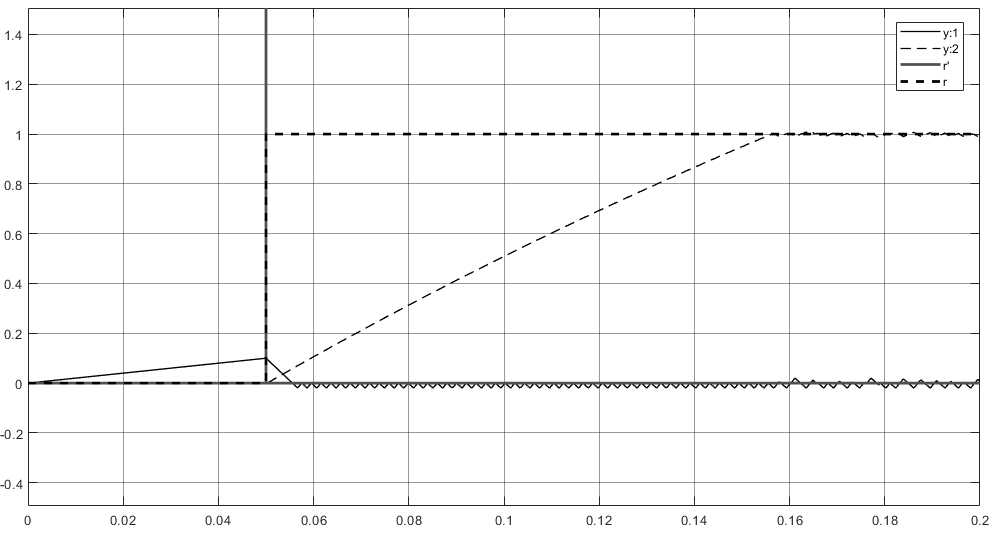
\includegraphics[width=0.9\linewidth]{1.png}
    \caption{График переходных процессов системы с сигнальной адаптацией}
    \label{fig:1}
\end{figure}

%%%%
%%%%
%%%%
\newpage
\section{Задание 2}

Объект управления описывается уравнением 

\[
0.25\ddot{y} + 0.4\dot{y} + y = 2u(t)
\]

Уравнение эталонной модели имеет вид:

\[
0.09\ddot{y_M} + 0.5\dot{y_M} + y_M = 3r(t)
\]

Закон управления задан в виде 

\[
u = {K_a}x(t) + k_b r(t)
\]

Преобразуем уравнения:
\[
\ddot{y} = -1.6\dot{y} -4y + 8u(t)
\]
\[
\mathbf{A} = \begin{bmatrix} 0 & 1 \\ -4 & -1.6 \end{bmatrix}, \quad
\mathbf{B} = \begin{bmatrix} 0 \\ 8 \end{bmatrix}.
\]


\[
\ddot{y_M} = - \frac{50}{9}\dot{y_M} - \frac{100}{9}y_M + \frac{300}{9}r(t)
\]
\[
\mathbf{A_M} = \begin{bmatrix} 0 & 1 \\ - \frac{100}{9} & - \frac{50}{9} \end{bmatrix}, \quad
\mathbf{B_M} = \begin{bmatrix} 0 \\ \frac{300}{9} \end{bmatrix}.
\]



\subsection*{Целевая функция}
\[
Q = \frac{1}{2} [y - y_M]^\top P [y - y_M],
\]
\[
\dot{Q} = [y - y_M]^\top P (Ay+Bu-A_My_M-B_Mr),
\]
\[
P = P^\top > 0
\]
\[
PA_M + A_M^\top P = -Q, Q = Q^\top > 0
\]
Пусть 
\[
\mathbf{Q} = \begin{bmatrix} 1 & 0 \\ 0 & 1 \end{bmatrix}, \quad
\mathbf{P} = \begin{bmatrix} p_1 & p_0 \\ p_0 & p_2 \end{bmatrix} + 
\]

Тогда
\[
\begin{bmatrix} p_1 & p_0 \\ p_0 & p_2 \end{bmatrix} \cdot{}
\begin{bmatrix} 0 & 1 \\ - \frac{100}{9} & - \frac{50}{9} \end{bmatrix} +  
\begin{bmatrix} 0 & - \frac{100}{9} \\  1 & - \frac{50}{9} \end{bmatrix}\cdot{}
\begin{bmatrix} p_1 & p_0 \\ p_0 & p_2 \end{bmatrix} = 
\begin{bmatrix} -1 & 0 \\ 0 & -1 \end{bmatrix} =>
\]

\[
\begin{bmatrix}
-\frac{100\,p_0 }{9} & -\frac{100\,p_2 }{9}\\
p_1 -\frac{50\,p_0 }{9} & p_0 -\frac{50\,p_2 }{9}
\end{bmatrix} + 
\begin{bmatrix}
0 & -\frac{100\,p_2 }{9}\\
p_1  & -\frac{50\,p_2 }{9}
\end{bmatrix} = 
\begin{bmatrix} -1 & 0 \\ 0 & -1 \end{bmatrix} =>
\]

\[
\begin{bmatrix}
-\frac{200\,p_0 }{9} & p_1 -\frac{50\,p_0 }{9}-\frac{100\,p_2 }{9}\\
p_1 -\frac{50\,p_0 }{9}-\frac{100\,p_2 }{9} & 2\,p_0 -\frac{100\,p_2 }{9}
\end{bmatrix} = 
\begin{bmatrix} -1 & 0 \\ 0 & -1 \end{bmatrix},
\]

Отсюда
\[
P = \begin{bmatrix} 1.34 & 0.045 \\ 0.045 & 0.0981 \end{bmatrix}
\]
Определитель P = 0.129 > 0.
Закон адаптивного управления:
\[
u = K_ax(t) + K_br(t)
\]
\[
\dot{K}_a(t) = -\gamma B^\top Pe(t) x^\top(t)
\]
\[
\dot{K}_b(t) = -\gamma B^\top Pe(t) r(t)
\]
Проведем моделирование в матлаб.
\subsection*{Моделирование в Simulink}

На рисунке 2 представлено сравнение графиков переходных процессов объекта управления (ОУ) и эталонной модели.
\begin{figure}[h]
    \centering
    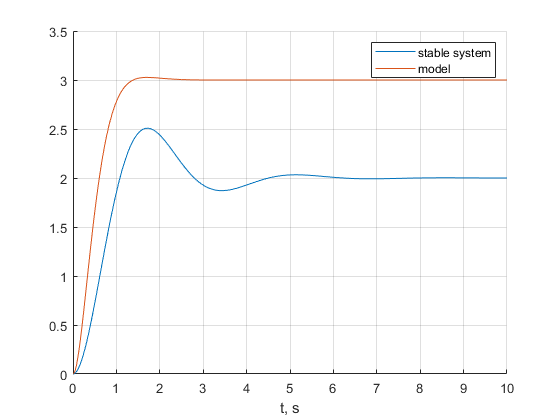
\includegraphics[width=0.9\linewidth]{2.png}
    \caption{Графики переходных процессов эталонной модели и ОУ}
    \label{fig:2}
\end{figure}

На рисунке 3 представлены график переходных процессов системы с параметрической адаптацией при разных значениях \[\gamma = (1, 10, 100)\].
\begin{figure}[h]
    \centering
    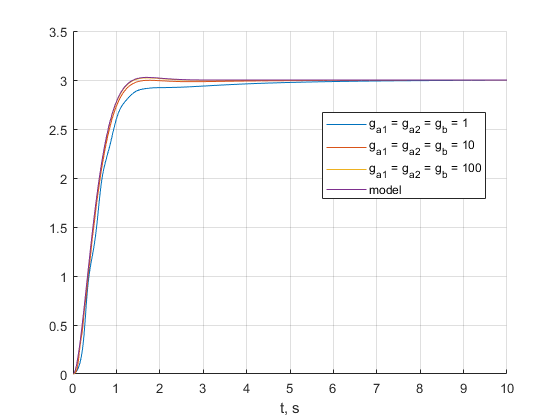
\includegraphics[width=0.8\linewidth]{3.png}
    \caption{График переходных процессов системы с параметрической адаптацией}
    \label{fig:3}
\end{figure}
Из рисунка 3 Видно, что при значении скорости адаптации 100 график переходного процесса эталонной модели перекрывает график переходного процесса ОУ. Целесообразно будет выбрать это значение в качестве оптимального по скорости адаптации.

На рисунке 4 представлен процесс адаптации на серии меандров. Видно что процесс почти завершается уже ко второму периоду.
\begin{figure}[h!]
    \centering
    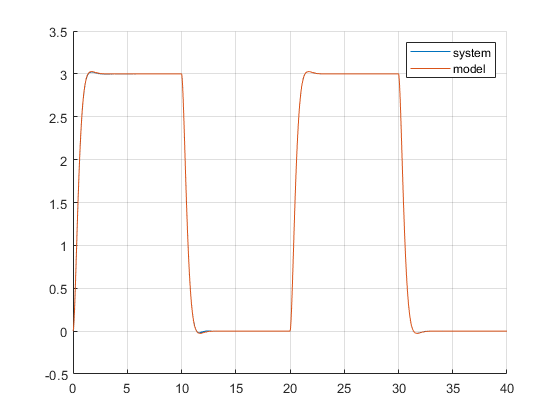
\includegraphics[width=0.8\linewidth]{4.png}
    \caption{График процесса адаптации}
    \label{fig:4}
\end{figure}

\newpage
На рисунке 5 показана структурная схема системы с параметрической адаптацией.
\begin{figure}[H]
    \centering
    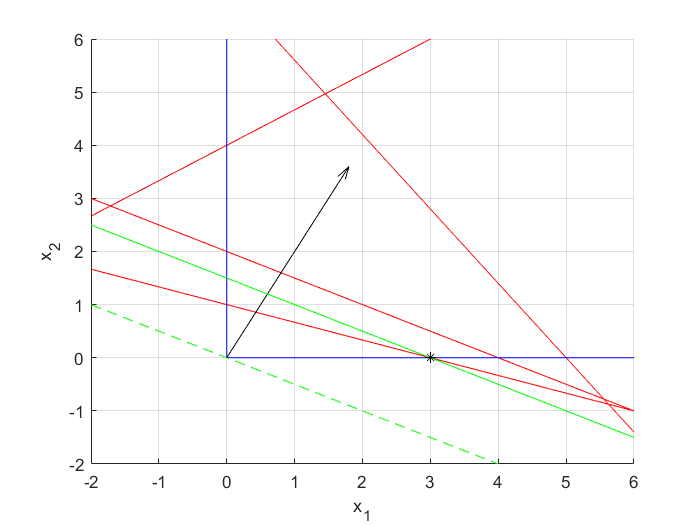
\includegraphics[width=0.8\linewidth]{5.png}
    \caption{Структурная схема системы}
    \label{fig:5}
\end{figure}




\newpage
\section{Задание 3}
\[
\begin{cases}
\dot{x} = -f_1(x) - f_2(y), \\
\dot{y} = f_3(x) - f_4(y),
\end{cases}
\]
\[
sign f_i(z)=sign(z), i = 1,2,3,4
\]
Рассмотрим функцию Ляпунова следующего вида:
\[
V(x, y) = \int_{0}^{x} f_3(x)\,dx + \int_{0}^{y} f_2(y)\,dy.
\]

\section*{Проверка положительной определенности}

Функция \(V(x, y)\) будет положительно определённой, если \(f_3(x)\) и \(f_2(y)\) имеют те же знаки, что и \(x\) и \(y\) соответственно. Так как интегралы этих функций увеличиваются с ростом \(|x|\) и \(|y|\), выполнены следующие условия:
\[
V(x, y) > 0 \quad \text{при } (x, y) \neq (0, 0), \quad V(0, 0) = 0.
\]
Таким образом, \(V(x, y)\) является положительно определённой функцией и подходит в качестве функции Ляпунова.

\section*{Вычисление производной функции Ляпунова}

Вычислим производную по времени \(V(x, y)\):
\[
\dot{V}(x, y) = \frac{\partial V}{\partial x} \dot{x} + \frac{\partial V}{\partial y} \dot{y}.
\]
Так как
\[
\frac{\partial V}{\partial x} = f_3(x), \quad \frac{\partial V}{\partial y} = f_2(y),
\]
то
\[
\dot{V}(x, y) = f_3(x) \dot{x} + f_2(y) \dot{y}.
\]

Подставим выражения для \(\dot{x}\) и \(\dot{y}\) из системы уравнений:
\[
\dot{x} = -f_1(x) - f_2(y), \quad \dot{y} = f_3(x) - f_4(y).
\]
Получаем:
\[
\dot{V}(x, y) = f_3(x) \big(-f_1(x) - f_2(y)\big) + f_2(y) \big(f_3(x) - f_4(y)\big).
\]

Раскроем скобки:
\[
\dot{V}(x, y) = -f_3(x)f_1(x) - f_3(x)f_2(y) + f_2(y)f_3(x) - f_2(y)f_4(y).
\]

Упростим выражение:
\[
\dot{V}(x, y) = -f_3(x)f_1(x) - f_2(y)f_4(y).
\]

\section*{Анализ знака производной}

\(-f_3(x)f_1(x)\) будет неположительным, так как \(\text{sign } f_i(x) = \text{sign } x\). Следовательно, \(f_3(x)f_1(x) > 0\).
Аналогично, \(-f_2(y)f_4(y) \leq 0\), так как \(f_i(y) = \text{sign } y\).

Таким образом:
\[
\dot{V}(x, y) \leq 0,
\]

\[
\dot{V}(x, y) < 0 \quad \text{при } (x, y) \neq (0, 0).
\]


Согласно теореме Ляпунова, если:
- \(V(x, y)\) положительно определена,
- \(\dot{V}(x, y)\) отрицательно определена,

то нулевое решение системы является асимптотически устойчивым.


\[
V(x, y) = \int_{0}^{x} f_3(x)\,dx + \int_{0}^{y} f_2(y)\,dy
\]
показывает, что нулевое решение системы
\[
\begin{cases}
\dot{x} = -f_1(x) - f_2(y), \\
\dot{y} = f_3(x) - f_4(y),
\end{cases}
\]
асимптотически устойчиво.


\end{document}

